\chapter{Implementation}

\section{Policy}
All aspects of a system using the Muen kernel must be specified in a policy XML
file. The policy is composed of the following main parts:

\begin{itemize}
	\item Hardware
	\item Kernel
	\item Binaries
	\item Subjects
	\item Scheduling
\end{itemize}

XML was chosen as a specification language since it is human-readable and can
be automatically verified against a schema. Furthermore, there is an existing
Ada library called XML/Ada TODO:Ref, which is opensource and freely available.

Since XML processing is not done by any trusted part of the system, the policy
contained in an XML file is transformed into SPARK source using the policy
compilation tool \texttt{skpolicy}. This process is described in detail in
section TODO:Ref.

Each of the main policy parts is presented in the following sections. Preceding
these descriptions is the specification of data types, which are the basis for
the subsequent definition of policy elements. The data types and elements map
directly to their corresponding XML schema definitions.

\subsection{Data types}
This section describes basic data types that are used in the specification of
the system policy. They are referenced in later chapters, illustrating different
parts of the policy.

\input{types.tex}

\subsection{Hardware}
\label{subsec:hardware}
\begin{figure}[h]
	\centering
	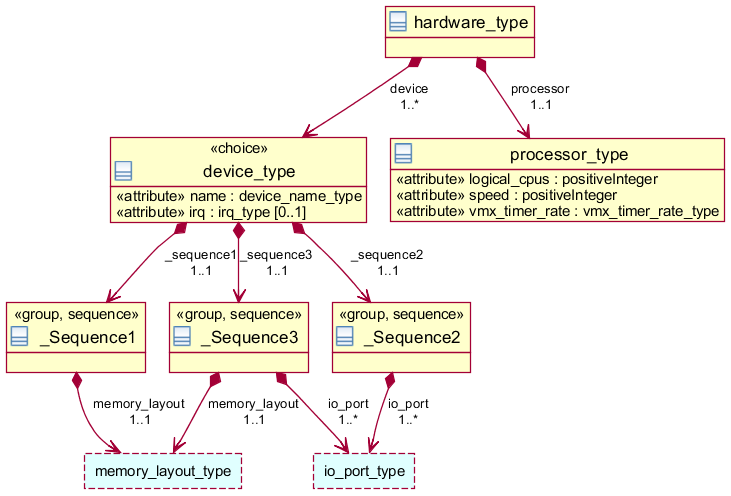
\includegraphics[width=\textwidth]{images/xml_hardware.png}
	\caption{Hardware policy}
\end{figure}
\input{hardware.tex}

\subsection{Kernel}
\begin{figure}[h]
	\centering
	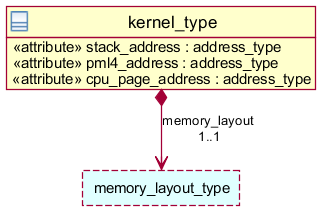
\includegraphics[scale=0.6]{images/xml_kernel.png}
	\caption{Kernel policy}
\end{figure}
\input{kernel.tex}

\subsection{Binaries}
\begin{figure}[h]
	\centering
	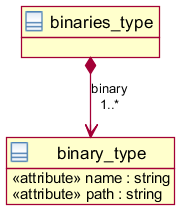
\includegraphics[scale=0.6]{images/xml_binary.png}
	\caption{Binaries policy}
\end{figure}
\input{binary.tex}

\subsection{Subjects}
\begin{sidewaysfigure}[hp]
	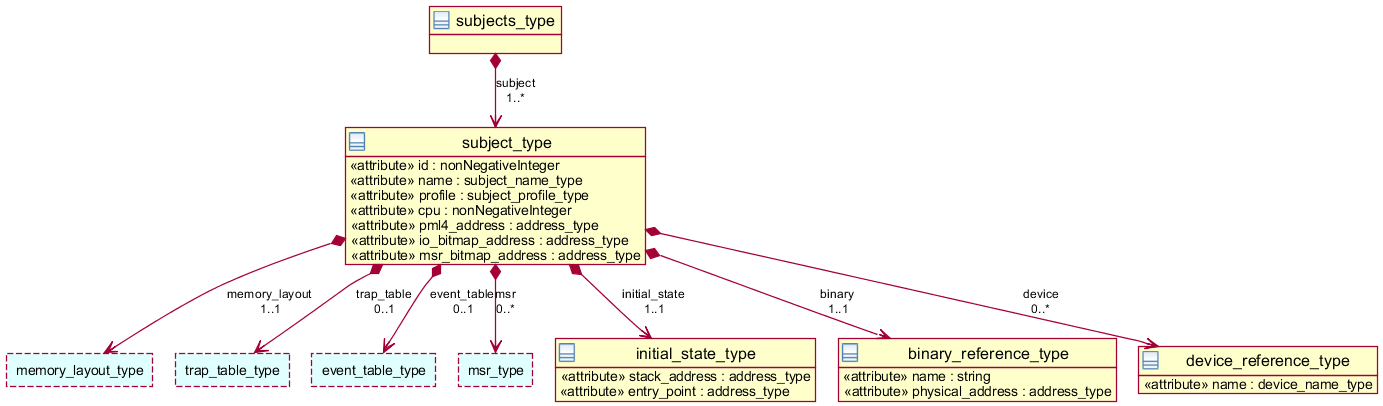
\includegraphics[width=\textwidth]{images/xml_subject.png}
	\caption{Subjects policy}
\end{sidewaysfigure}
\input{subject.tex}

\subsection{Scheduling}
\begin{figure}[h]
	\centering
	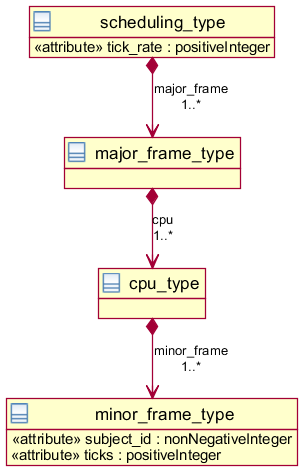
\includegraphics[scale=0.6]{images/xml_scheduling.png}
	\caption{Scheduling policy}
\end{figure}
\input{scheduling.tex}


\section{Kernel}
\subsection{Init}\label{subsec:init}
After reset of a x86 system, the processor begins executing code at physical
address \texttt{ffff:0000}, which is mapped to the PC
BIOS\index{BIOS}\footnote{Basic Input/Output System}. The BIOS first performs
tests and initialization routines and then searches for a bootable storage
media. If found, the BIOS copies the first sector of the storage media to
physical address \texttt{0000:7C00} and jumps to this address (i.e. starts
executing code at this address). This is where the system bootloader comes to
live which is responsible to boot operating systems according to its
configuration. Many bootloaders first load additional code from the storage
media and then prepare the environment for OS execution.

The Muen seperation kernel is compliant to the multiboot specification, version
0.6.96 \cite{multiboot}. The multiboot standard is used to uniformly boot
different operating system kernels by multiboot-aware bootloaders.
The Muen kernel exports the required multiboot header within the first 8192
bytes of the OS image. The bootloader loads the OS image into memory according
to the information found in the header and jumps to the physical kernel entry
point specified in this header.

It is the bootloader's task to prepare the system state as demanded by the
multiboot standard, see \cite{multiboot} section 3.2 for details. The system
kernel can except the system to be in this state. After the Muen kernel comes to
live, it performs additional steps before jumping into the main SPARK kernel.
This initial startup code is written in Assembly and conducts the following
tasks:
\begin{enumerate}
	\item Copy the AP trampoline to low-memory, see section
		\ref{subsec:mp-support} \item Initialize per-CPU VMXON regions
	\item Initialize subject VMCS regions
	\item Enable PAE\index{PAE}\footnote{Physical Address Extension}
	\item Initialize per-CPU kernel pagetables
	\item Enable IA-32e mode and execute-disable (NX)
	\item Enable paging, write protection, caching and native FPU error
		reporting
	\item Set up 64-bit GDT\index{GDT}\footnote{Global Descriptor Table}
	\item Set up Page-Attribute Table (PAT)
	\item Set up kernel stack
	\item Initialize Ada runtime
	\item Jump into kernel main
\end{enumerate}
After this initial steps are executed, the system is in 64-bit IA-32e mode and
all prerequisites are met to enable VMX root operation.

\subsection{Scheduling}
\begin{figure}[h]
	\centering
	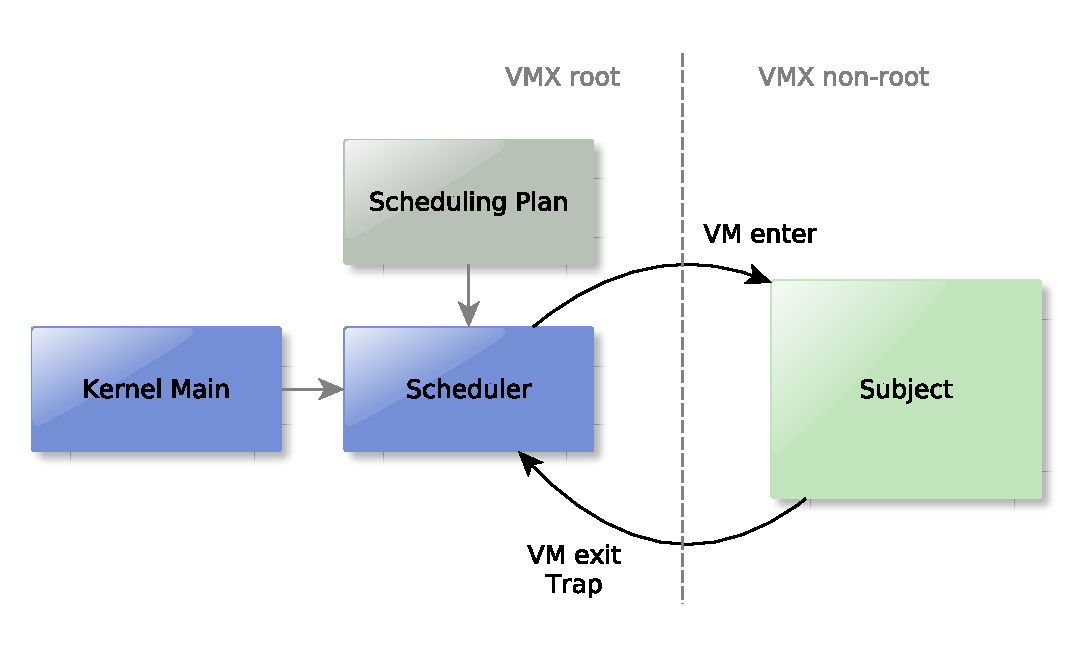
\includegraphics[scale=0.6]{images/scheduler-overview}
	\caption{Kernel scheduler}
	\label{fig:scheduler-overview}
\end{figure}

\subsection{Traps}
\subsection{Exceptions and Interrupts}
\begin{figure}[h]
	\centering
	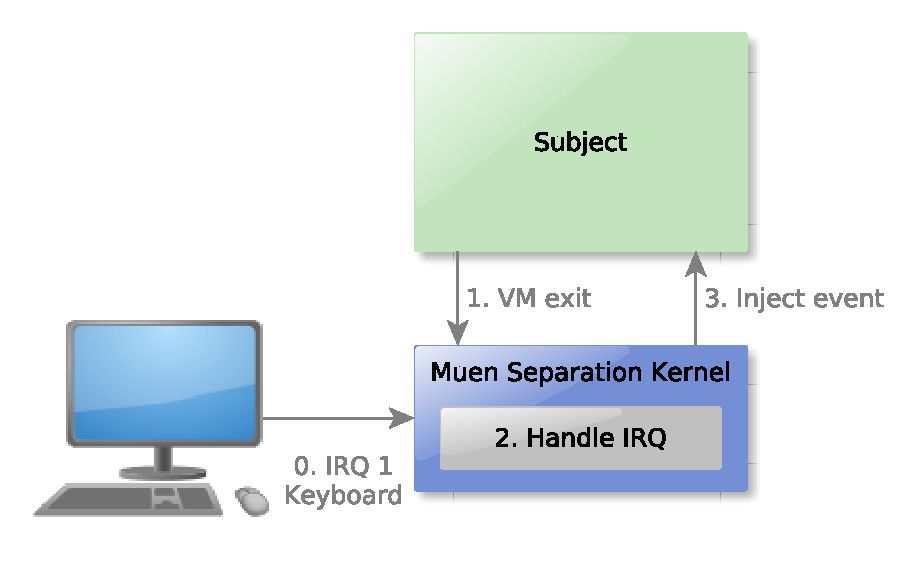
\includegraphics[scale=0.6]{images/external-interrupt}
	\caption{External interrupt handling}
	\label{fig:external-interrupt}
\end{figure}

\subsection{Multicore support}\label{subsec:mp-support}
The Muen separation kernel makes use of all logical processors available in a
system. The processor count of a specific hardware platform is specified in the
system policy, see section \ref{subsec:hardware}. This section describes how the
multicore setup is done on kernel startup.

Modern PC systems comply to the Intel MultiProcessor (MP\index{MP})
specification. In short, the Intel MP specification is an open-standard
describing enhancements to both operating systems and firmware to be able to
init, boot and operate x86 multiprocessor systems. For more information see
\cite{intel:mp}.

After the hardware completed its part of the MP specification, one processor
has been negotiated to be the bootstrap processor (BSP\index{BSP}). All other
logical processors, called application processors (AP\index{AP}), halt until
they receive a specific inter-processor interrupt (IPI\index{IPI}) sequence.

\begin{figure}[h]
	\centering
	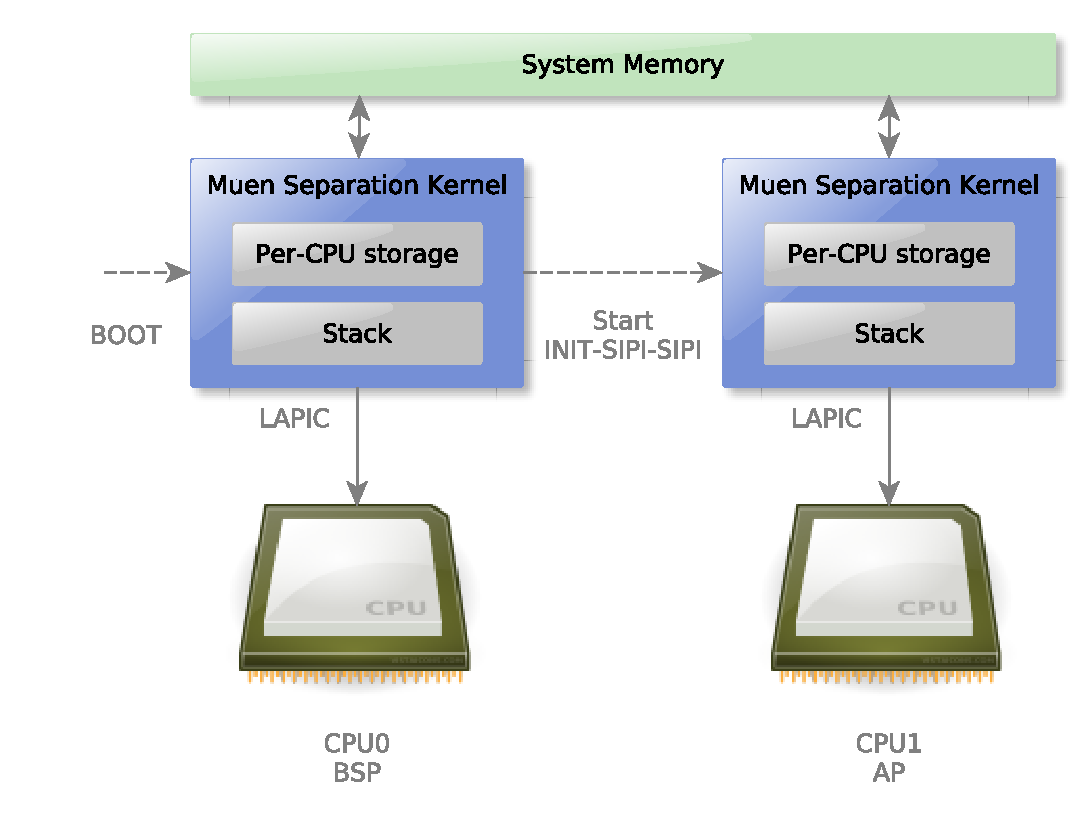
\includegraphics[scale=0.6]{images/mp-overview}
	\caption{Multicore architecture}
	\label{fig:mp-overview}
\end{figure}

The BSP starts executing code as describe in section \ref{subsec:init}. The
init code initializes the system and jumps into the main SPARK kernel. The
kernel running on the BSP is responsible to bootstrap the other application
processors. It first enables its local APIC\index{APIC} to be able to send
inter-processor interrupts to the halted AP processors. To wakeup the APs, the
INIT-SIPI-SIPI IPI sequence must be sent to their APICs, as described in the MP
specification. See also figure \ref{fig:mp-overview} for an illustration of
this process. The SIPI IPI contains the physical address vector of the
trampoline code copied to low-memory by the init code. The AP processors jump
to this code after wakeup. The trampoline performs the following steps:

\begin{enumerate}
	\item Set up 32-bit GDT\index{GDT}
	\item Switch CPU to protected mode
	\item Initialize DS and SS segments
	\item Jump to the AP entry point in the init code
\end{enumerate}

These steps initialize the APs to the same architectural state as the
bootloader did for the BSP: 32-bit protected mode with paging disabled.
Therefore, the final step is to let the AP processors jump to the identical
init code described in section \ref{subsec:init}.

\subsubsection{Per-kernel memory}
The Muen kernels operate fully symmetrical, i.e. code running on the different
logical processors is (binary) identical. Nevertheless, each kernel owns a
distinct stack page and also a page to store per-CPU data. This however is fully
transparent to the kernels as their virtual stack and global storage addresse
values are the same. This is achieved by using different page table structures
for each kernel. Page tables are created by the policy tool and setup on system
startup by the init code. The main kernel has no access to these structures in
memory and does not bother with memory management.

\subsubsection{Synchronization} Since synchronization is error-prone and it is
desirable to reduce inter-core dependencies as much as possible, the Muen
kernel tries to avoid locks and other synchronization primitives. Nevertheless
minimal synchronization is required at certain key points in the code. This
section describes the spinlock and barrier mechanisms used by the kernel.

\paragraph{Spinlock}
The spinlock implementation uses the \texttt{XCHG} processor instruction to
atomically swap the value one with the contents of a lock variable in memory.
If the result of the set operation is zero, no other core currently holds the
lock and it is successfully acquired. If the result is one, the lock is
currently busy and the core must spin and retry again.

Inside the lock's busy loop the \texttt{PAUSE} instruction is used to improve
performance and resource utilization on CPUs with hyper-threading
(HTT\index{HTT}) enabled TODO:REF.

\paragraph{Barrier}
As described in section \ref{subsec:scheduling}, to guarantee temporal
separation, the scheduling plans on the different logical processors must be
synchronized on major frame transition.

This is achieved by ...

\subsection{Events}
\begin{figure}[h]
	\centering
	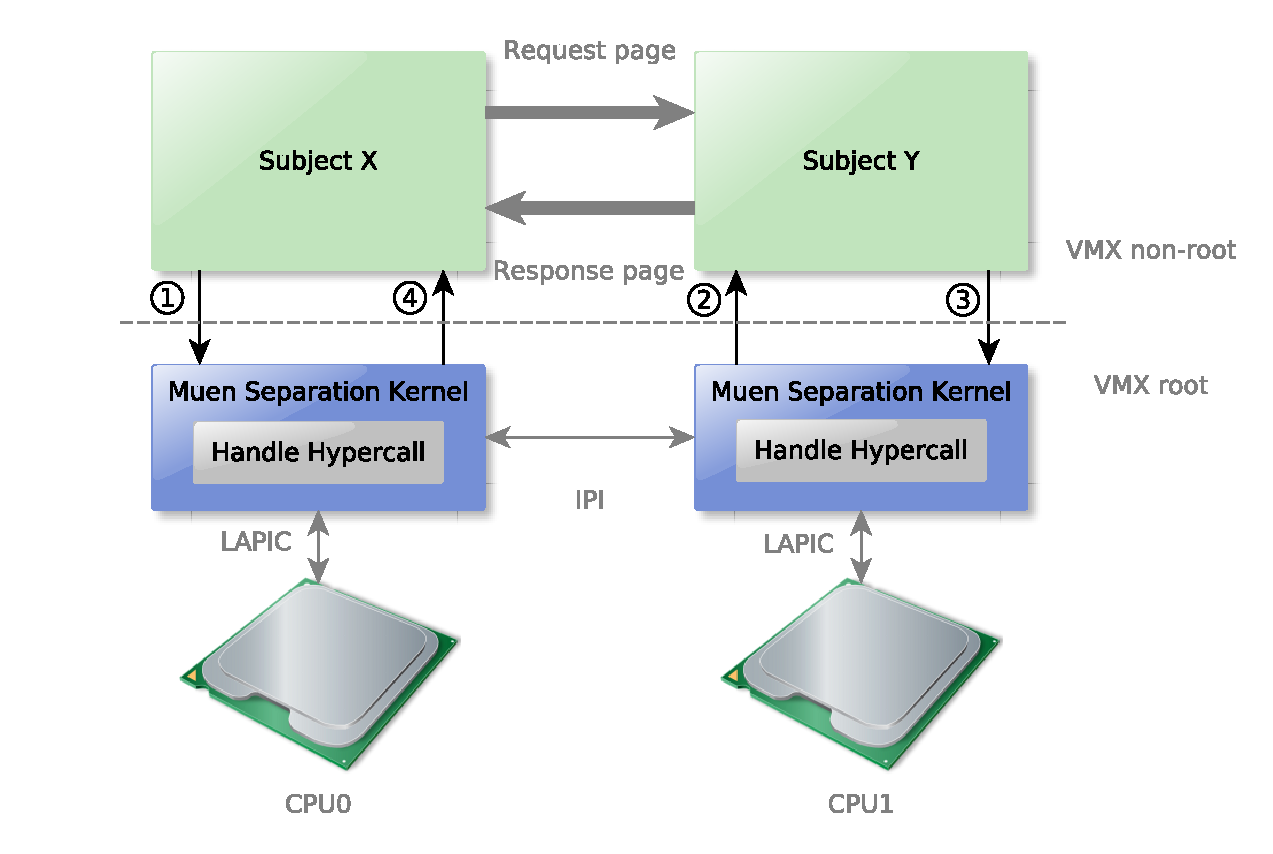
\includegraphics[width=\textwidth]{images/inter-core-events}
	\caption{Inter-core events}
	\label{fig:inter-core-events}
\end{figure}

\section{Build}
TODO: explain the complete process, target dependencies and implemented tools.

\subsection{Policy compilation}
The \texttt{skpolicy} tool compiles the XML system policy outlined in section
\ref{sec:policy} to different output formats as shown in figure
\ref{fig:policy-compilation}.

\begin{figure}[h]
	\centering
	\begin{tikzpicture}
		\node (pol) [greenbox]                            {Policy};
		\node (skp) [apribox, below=of pol]               {skpolicy};
		\node (sou) [bluebox, below=of skp, xshift=1.5cm] {Source specs};
		\node (pag) [bluebox, left=of sou]                {Page tables};
		\node (iob) [bluebox, left=of pag]                {I/O bitmaps};
		\node (msr) [bluebox, right=of sou]               {MSR bitmaps};

		\draw[arrow] (pol) to (skp);
		\draw[arrow] (skp) to (sou);
		\draw[arrow] (skp) to (msr);
		\draw[arrow] (skp) to (pag);
		\draw[arrow] (skp) to (iob);
	\end{tikzpicture}
	\caption{Policy compilation}
	\label{fig:policy-compilation}
\end{figure}

The generated subject page tables, I/O and MSR bitmaps are included in the final
system image by the \texttt{skpacker} utility explained in the following section
\ref{subsec:image-packaging}. These files are all in binary form and correspond
to the format mandated by the respective Intel SDM chapters (TODO:REF). Page
tables are generated for subjects as well as for the kernel itself.

The generated SPARK and Assembly source specifications are included in the
kernel directly. These specifications provide the kernel with the following
information:

\begin{itemize}
	\item \emph{IRQ routing specification}\\
		Used by the kernel to program the system's I/O APIC for interrupt
		routing.
	\item \emph{Kernel address constants}\\
		Define kernel stack, page table and per-CPU storage memory addresses.
	\item \emph{Scheduling plans for all CPU cores}\\
		The scheduling plans are indexed by the logical processor's APIC ID.
		Each kernel copies its associated scheduling plan to the per-CPU storage
		area on initialization.
	\item \emph{Subjects specification}\\
		Defines all subjects and their parameters, see policy section
		\ref{subsec:subjects}.
	\item \emph{Packer specification}\\
		Defines the configuration used for the \texttt{skpacker} tool outlined
		in the following section \ref{subsec:image-packaging}.
\end{itemize}

\subsection{Subject binary analysis}\label{subsec:subject-binary-analysis}
The \texttt{skconfig} tool uses the Binary File Descriptor (BFD\index{BFG})
library to analyze subject binaries and creates appropriate XML\index{XML}
policy specifications from it, see figure \ref{fig:object-analysis}. This is
useful to generate the initial state and the memory layout directly from a
native subject binary instead of writing it by hand. The tool extracts stack
address, entry point and memory layout from a subject binary.

\begin{figure}[h]
	\centering
	\begin{tikzpicture}
		\node (obj) [bluebox]                {Binary object};
		\node (skc) [apribox,  below=of obj] {skconfig};
		\node (xml) [greenbox, below=of skc] {XML specification};

		\draw[arrow] (obj) to (skc);
		\draw[arrow] (skc) to (xml);
	\end{tikzpicture}
	\caption{From binary object to XML specification}
	\label{fig:object-analysis}
\end{figure}

The exctracted subject initial state and memory layout XML specifications can be
included in the system policy before compilation by the \texttt{skpolicy} tool.
The generated memory layout is only as permissive as required by the original
subject binary. For example, the memory region mapped for executable code
(the \texttt{.text} section) will be executable but non-writeable. This is in
contrast to just providing a big enough memory region with all permissions to
the subject with no exact mapping of binary sections to memory access
permissions (i.e. read, write, execute).

\subsection{Image packaging}\label{subsec:image-packaging}
The \texttt{skpacker} tool is responsible to assemble the final bootable system
image from the parts produced in the previous build steps. Figure
\ref{fig:image-packaging} illustrates the process. The tool includes the special
packer source specification created from the system policy. This specification
includes information about subject binaries and their physical address in the
final image.

\begin{figure}[h]
	\centering
	\begin{tikzpicture}
		\node (knl) [bluebox]                              {Kernel binary};
		\node (sub) [bluebox, left=of knl]                 {Subject binaries};
		\node (pag) [bluebox, left=of sub]                 {Page tables};
		\node (bit) [bluebox, right=of knl]                {Bitmaps};
		\node (skp) [apribox, below=of knl, xshift=-1.5cm] {skpacker};
		\node (spe) [bluebox, left=of skp]                 {Packer spec};
		\node (sys) [greenbox, below=of skp]               {System image};

		\draw[arrow] (pag) to (skp);
		\draw[arrow] (sub) to (skp);
		\draw[arrow] (knl) to (skp);
		\draw[arrow] (bit) to (skp);
		\draw[arrow] (skp) to (sys);
		\draw[arrow] (spe) to (skp);
	\end{tikzpicture}
	\caption{System image packaging}
	\label{fig:image-packaging}
\end{figure}

The remaining configuration is extracted from the source specification provided
to the kernel. Listing \ref{lst:skpacker} shows the output of a
\texttt{skpacker} run with the example system described in section
\ref{sec:example-system}. The fist column in the output designate physical
addresses in memory. The second column specifies the type of the packaged file
at this specific memory location. The abbreviations have the following meaning:

\begin{itemize}
	\item \emph{PML4} The file at this address designates a page table
		structure. It is either a page table for a kernel or for a subject. The
		kernels running on the different logical processors have different page
		tables to allow distinct stack and per-CPU storage pages transparently.
	\item \emph{IOBM} The file is a subject I/O bitmap. Specifies which I/O
		ports a subject is allowed to access.
	\item \emph{MSBM} The file is a subject MSR bitmap. Specifies which MSRs a
		subject is allowed to access.
	\item \emph{BIN} The file is a subject (raw) binary.
\end{itemize}

\begin{lstlisting}[
	caption=Example output of skpacker tool,
	label=lst:skpacker,
	frame=none,
	numbers=none]
         Packaging kernel image 'obj/kernel'
         0000000000200000 [PML4] kernel (0)
         0000000000204000 [PML4] kernel (1)
         0000000000208000 [PML4] kernel (2)
         000000000020c000 [PML4] kernel (3)
         0000000000210000 [PML4] tau0
         0000000000214000 [IOBM] tau0
         0000000000216000 [MSBM] tau0
         0000000000217000 [BIN ] tau0
         0000000000240000 [PML4] vt
         0000000000244000 [IOBM] vt
         0000000000246000 [MSBM] vt
         0000000000247000 [BIN ] vt
         0000000000270000 [PML4] crypter
         0000000000274000 [IOBM] crypter
         0000000000276000 [MSBM] crypter
         0000000000277000 [BIN ] crypter
         00000000002a0000 [PML4] sm
         00000000002a4000 [IOBM] sm
         00000000002a6000 [MSBM] sm
         00000000002a7000 [BIN ] sm
         00000000002d0000 [PML4] xv6 (EPT)
         00000000002d4000 [IOBM] xv6
         00000000002d6000 [MSBM] xv6
         00000000002d7000 [BIN ] xv6
\end{lstlisting}

\section{Example system}\label{sec:example-system}
\begin{figure}[h]
	\centering
	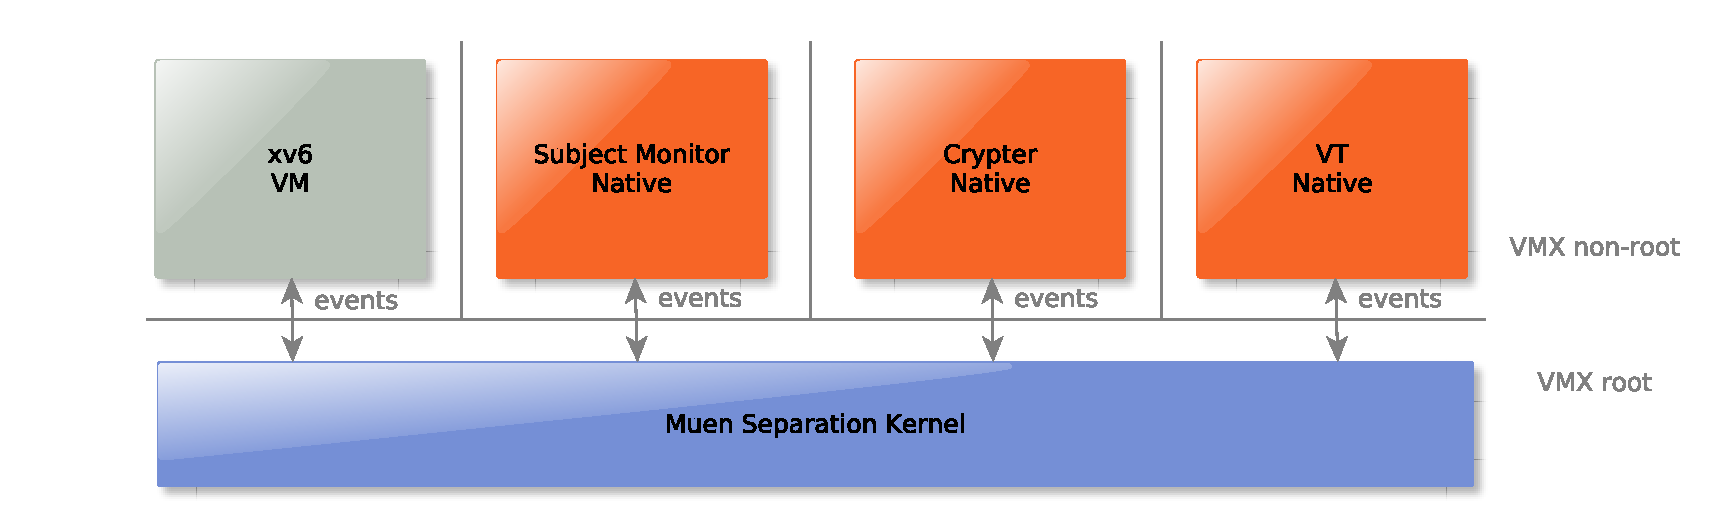
\includegraphics[width=\textwidth]{images/architecture-example_system}
	\caption{Example system}
	\label{fig:example-system}
\end{figure}
